\documentclass[12pt]{article}

%-------------PACKAGES------------- 
\usepackage[margin=1in]{geometry} 
\usepackage{amsmath,amsthm,amssymb}
\usepackage{pgfplots}
\usepackage{float}
\usepackage{braket}
\usepackage{titling}
\usepackage{wrapfig}
\usepackage{tikz}
\usepackage{mwe}
\usepackage{enumitem}
\usepackage{mathtools}
\usepackage{scrextend}
\usepackage{listings}
\usepackage{color}
\usepackage{caption}
\usepackage{subcaption}
\usepackage{algorithm,algpseudocode}
\usetikzlibrary{shapes,arrows,chains}
\usetikzlibrary[calc]

%-------------FORMATTING-------------
\setlength{\droptitle}{-7.5em} 
\setlength{\parindent}{0pt}
\def\LW{\dimexpr.25\linewidth-.5em} 
\tikzstyle{line} = [draw, -latex']
 
%--------------COMMANDS--------------
\newcommand{\N}{\mathbb{N}}
\newcommand{\Z}{\mathbb{Z}}
\newcommand{\R}{\mathbb{R}}
\newcommand{\C}{\mathbb{C}}
%\renewcommand{\qedsymbol}{\filledbox}

\DeclarePairedDelimiter \abs{\lvert}{\rvert}%
\DeclarePairedDelimiter \babs{\bigg\lvert}{\bigg\rvert}%
\DeclarePairedDelimiter \norm{\lVert}{\rVert}%

%------------ENVIRONMENTS------------- 
\newenvironment{theorem}[2][]{\begin{trivlist}
\item[{\bfseries #1}\hskip \labelsep {\bfseries #2.}]}{\end{trivlist}}
\newenvironment{lemma}[2][Lemma]{\begin{trivlist}
\item[\hskip \labelsep {\bfseries #1}\hskip \labelsep {\bfseries #2.}]}{\end{trivlist}}
\newenvironment{exercise}[2][Exercise]{\begin{trivlist}
\item[\hskip \labelsep {\bfseries #1}\hskip \labelsep {\bfseries #2.}]}{\end{trivlist}}
\newenvironment{reflection}[2][Reflection]{\begin{trivlist}
\item[\hskip \labelsep {\bfseries #1}\hskip \labelsep {\bfseries #2.}]}{\end{trivlist}}
\newenvironment{proposition}[2][Proposition]{\begin{trivlist}
\item[\hskip \labelsep {\bfseries #1}\hskip \labelsep {\bfseries #2.}]}{\end{trivlist}}
\newenvironment{corollary}[2][Corollary]{\begin{trivlist}
\item[\hskip \labelsep {\bfseries #1}\hskip \labelsep {\bfseries #2.}]}{\end{trivlist}}
\newenvironment{definition}[2][]{\begin{trivlist}
\item[{\bfseries #1}\hskip \labelsep {\bfseries #2.}]}{\end{trivlist}}
\theoremstyle{remark}
\newtheorem*{remark}{Remark}

%-------------CODE-STYLE------------
\definecolor{dkgreen}{rgb}{0,0.6,0}
\definecolor{gray}{rgb}{0.5,0.5,0.5}
\definecolor{mauve}{rgb}{0.58,0,0.82}
\lstset{frame=tb,
	language=C++,
	aboveskip=3mm,
	belowskip=3mm,
	showstringspaces=false,
	columns=flexible,
	basicstyle={\small\ttfamily},
	numbers=none,
	numberstyle=\tiny\color{gray},
	keywordstyle=\color{blue},
	commentstyle=\color{dkgreen},
	stringstyle=\color{mauve},
	breaklines=true,
	breakatwhitespace=true,
	tabsize=3
}

\tikzset{
	path image/.style={
		path picture={
			\node at (path picture bounding box.center) {
				\includegraphics[height=3cm]{example-image}};}},
	path tikzimage/.style={
		path picture={
			\node at (path picture bounding box.center)
			[circle, fill=blue!50, scale=2, text=yellow]{Bravo};}}
}
	
\lstset{
	morekeywords={end}
}

%------------------------------------ 
%---------START-OF-DOCUMENT----------
%------------------------------------
\begin{document}
 
\title{Paper Summary}
\author{David Miller \\ 
CIS 5930: Social Network Mining} 

\maketitle

A Graph Cluster is a graph $G^\prime \subseteq G = \{V,E\}$ that it is partitioned into sets $C = \{C_1, \dots, C_n\}$ such that $C_i \cap C_j = \emptyset$ for any $i \neq j = 1, \dots, n$. The graph $G$ is the original graph of data input. If the clustering algorithm breaks edges between vertices in different clusters then $G^\prime \subsetneq G$ since $e_{i,j} \not\in G^\prime$ for $v_i \in C_m, v_j \not\in C_m$. The main gaol of clustering algorithms are to identify clusters of densely linked nodes given only the graph itself. However, in many cases we only care about a cluster that pertains to a set of nodes $S = \{v_1, \dots, v_k\}$. This is where local graph clustering comes into play. Local graph clustering is a specific case that takes an additional input in the form of a seed set of vertices. The idea is to identify a single cluster nearby the seed set without ever exploring the entire graph, which makes the local clustering methods much faster than their global counterparts \cite{paper}. 
\begin{wrapfigure}{l}{0.5\textwidth}
	\vspace{-15pt}
	\hspace{0pt}
	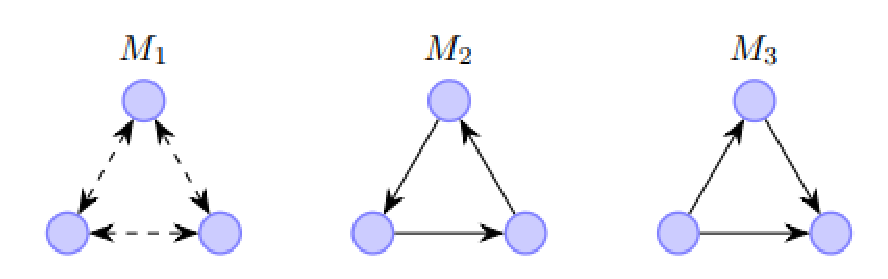
\includegraphics[height=2.5cm,width=0.5\textwidth]{fig1.eps}
	\\
	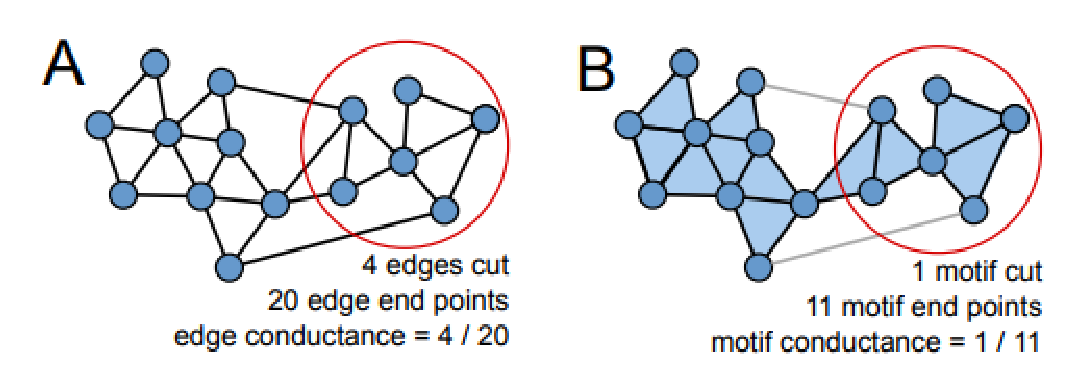
\includegraphics[height=2.5cm,width=0.5\textwidth]{fig2.eps} 
	\caption{}
	\vspace{-14pt}
\end{wrapfigure} 
The method in the paper cares not only about undirected graphs, but also directed graphs. Therefore the method searches for motifs as a measure for clustering nodes together. A motif is a characteristic or property that the graph may have. Examples in figure 1 (upper) include a triangle in any direction, a cycle , and a feed forward loop. The lower half of figure one shows a "classical" clustering cut with conductance measure 4/20 (left) versus a triangle motif cut with conductance measure 1/11 (right). We want the conductance measure to essentially be zero since its a heuristic metric on how much we are separating a node to its respective cluster. The cluster found in figure 1 is due to seeding the algorithm with at least one vertex from that cluster. The triangle motif clearly uncovers the cluster better than the "classical" edge density approach. Due to the mathematical nature of the paper, it would be best now to just talk about the advantages of the method talked about in the paper and look at some results. In terms of advantages, the method runs in $\mathcal{O}(\frac{1}{\epsilon(1-\alpha)})$, where $1 - \alpha$ is the probability of the random walker "teleporting" back to a seed node $u$ and $\epsilon$ is some prescribed tolerance. Essentially, since the algorithm performs local clustering rather than global, the time required to uncover some cluster $C^*$ with a given set of seeds $S^* \subseteq C^*$ requires less time than efficient global clustering algorithms. For the experiments, a planted partition model and LFR model was used with respective $F1$ scores. The planted partition model generates
an undirected unweighted graph with $kn_1$ nodes. Nodes are partitioned into $k$ built-in communities, each of size $n_1$. Between any
pair of nodes from the same community, an edge exists with probability $p$ and between any pair of nodes from different communities,
an edge exists with probability $q$. Each edge exists independently
of all other edges \cite{paper}. The LFR model also generates random 

\begin{wrapfigure}{r}{0.5\textwidth}
	\vspace{-15pt}
	\hspace{0pt}
	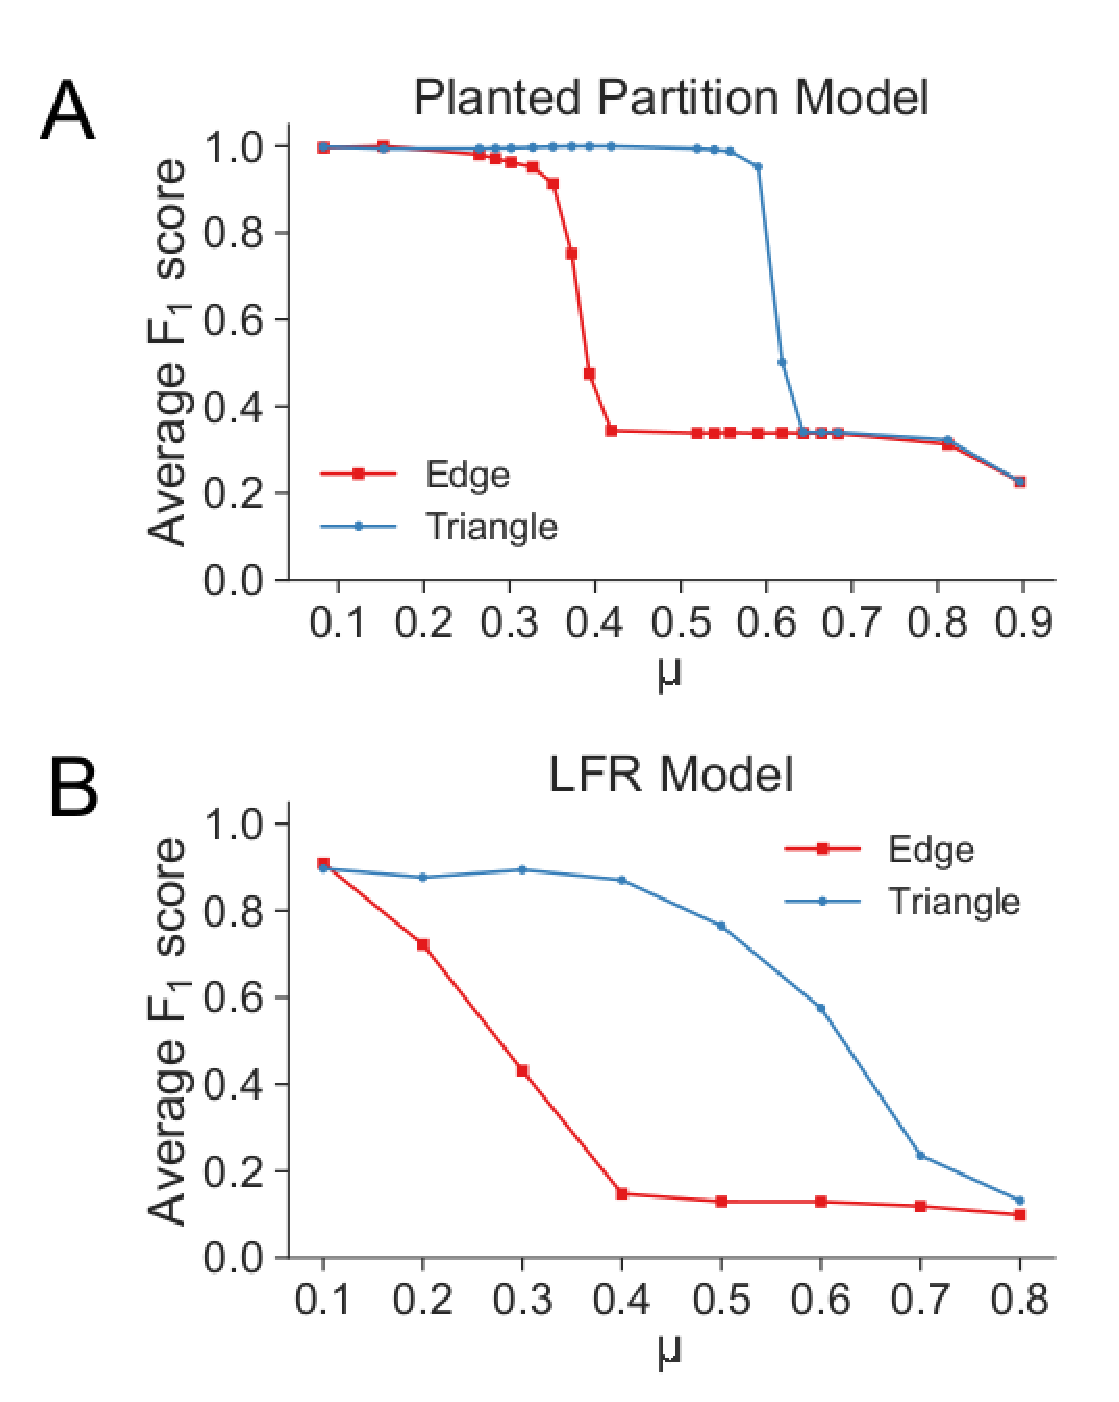
\includegraphics[height=10cm,width=0.5\textwidth]{fig3.eps}
	\caption{}
	\vspace{-14pt}
\end{wrapfigure} 

graphs with planted communities, but the model is designed to capture several properties of real-world networks with community structure such
as skew in the degree and community size distributions and overlap
in community membership for nodes \cite{complementary}. The $F_1$ scores is a measure of the method's accuracy. The results in figure 2 compare the method in the paper using triangle motifs and some set of seeds determined algorithmically versus a "classical" clustering algorithm using edge density. the $x-axis$ is the mixing parameter $\mu$, which specifies the fraction of neighbors of a node that cross cluster boundaries. Not much improvement is made when clusters are easily identifiable ($\mu << 1$) or when clusters are highly entangled with each other ($\mu >> 0$). However, when clusters are not so intertwined or easily identifiable then the method in the paper severely outperforms classical approaches. These types of results make it suitable for consumer based clustering and allow for future work to head in this direction. Examples of this include Netflix using local clustering with seeds as user's movies and shows watched, Amazon using local clustering with using purchased items as seeds, and Spotify using local clustering with using songs listened to as seeds. As long as there are recommendation systems local clustering will have an application. \\

Three strengths I found with the paper are
\begin{enumerate}
	\item The use of seeds allows for one to uncover a particular cluster of interest rather than clustering globally and picking them out.
	\item Due to local clustering rather than global, it runs very fast and allows for scalability.
	\item The use of motifs allows the user to detect clusters based on a measurement of interest.
\end{enumerate} 
\vspace{0.5cm}

Three weaknesses I found with the paper are
\begin{enumerate}
	\item The results only compare the method to one other method which may imply there are "classical" global algorithms that may not have better time complexity but may have better $F1$ scores.
	\item The search for good seeds is a global algorithm rather than local.
	\item There may exist poor choices of motifs that may produce poor results. 
\end{enumerate}
\vspace{0.5cm}

Questions for the reader
\begin{enumerate}
	\item Could the algorithm be used iteratively to cluster globally? IF so will it be faster than currently existing global clustering algorithms?
	\item Why does the algorithm perform only as good as the edge clustering algorithm when $\mu << 1$ or $\mu >> 0$?
\end{enumerate}
\vspace{0.5cm}

\begin{thebibliography}{unsrt}
	\bibitem{paper}
	Hao Yin, Austin R. Benson, Jure Leskovec, David F. Gleich, \emph{Local Higher-Order Graph Clustering}, KDD’17, August 13-17, 2017, Halifax, NS, Canada.
	\bibitem{complementary}
	A. Lancichinetti and S. Fortunato. \emph{Benchmarks for testing community detection algorithms on directed and weighted graphs with overlapping communities}. Physical Review E, 2009.
\end{thebibliography}

\end{document}